\documentclass{../../../../style/mkimain}

\series{2}
\month{březen}
\year{2023}

\begin{document}
\ExecuteMetaData[../../problems/problem2-A/problem2-A.tex]{header}
\noindent\ExecuteMetaData[../../problems/problem2-A/problem2-A.tex]{task}
\proborigin{}
\klein
Venuše nemá vlastní magnetické pole, takže na první pohled by se mohlo zdát, že odpověď je jasná - Ne, žádný jev podobný zemské polární záři v 
atmosféře Venuše pozorovat nelze, protože nabité částice slunečního větru nemají s čím interagovat.

Tato úvaha je zcela správná, ale i přes to astronomové pozorují \emph{auroru} na Venuši.
\begin{figure}[htpb]
    \begin{center}
    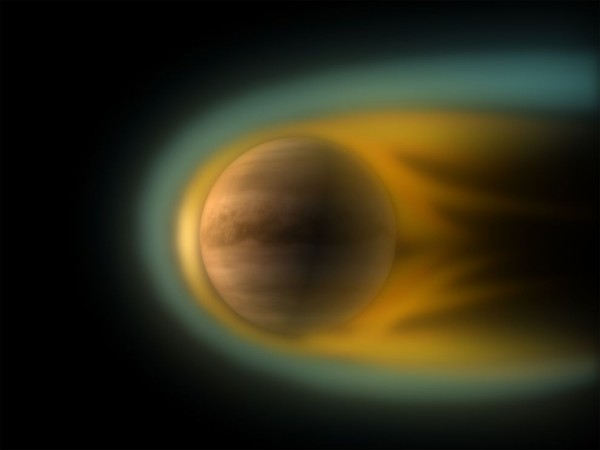
\includegraphics[width=7cm]{images/venus-aurora.jpg}
    \\
    \emph{Aurora} na Venuši\footnotemark
    \end{center}
\end{figure}
\footnotetext{Illustration by C. Carreau/ESA}
\\ Jak je to možné? V atmoféře Venuše se vyskytuje hodně iontů, převážně ionty kyslíku \ce{O^{2-}}. Plazmoid blížíce se k Venuši indukuje v 
ionosféře Venuše slabé magnetické pole. Nabité částice slunečního větru pak s tímto indukovaným polem interagují a předávájí svojí energii 
kyslíkovým iontům, které jí následně vyzáří a vytvoří tak v celé atmosféře jev podobný polární záři na Zemi. 
\end{document}
